\section{Experiments}
\label{sec:experiments}

\paragraph{Setup.}
We evaluate on two benchmarks, both split into B0Inc20: 10 tasks of 20
classes each, 200 classes in total.
\begin{itemize}
  \item \emph{ImageNet-R}~\cite{hendrycks2021many}: the fixed split with
    23\,918 training and 6\,082 test images.
  \item \emph{ImageNet-A}~\cite{hendrycks2021nae}: an 80/20 split per class
    with seed 67, about 6\,000 training and 1\,500 test images, i.e.\ roughly
    30 training images per class.
\end{itemize}
RSIAT uses its published configuration: SGD with batch size 48 and 30/30
epochs (ImageNet-R) or 20/15 epochs (ImageNet-A) for the base and incremental
tasks, and 10 CA epochs. We report the average incremental accuracy (AIA)
over the 10 stages and the final accuracy. All runs used one NVIDIA RTX PRO
6000 Blackwell GPU, PyTorch 2.11 and CUDA 12.8, with three runs in parallel.
In total there are 11 runs, each evaluating all heads:
\begin{itemize}
  \item tuning group: ImageNet-R, seed 1993, three replicates;
  \item held-out: ImageNet-R, seeds 2015, 2026 and 2042;
  \item held-out: ImageNet-A, seed 1993 (three replicates), 2015 and 2026.
\end{itemize}
In every run, the training curve is bit-identical to that of the plain RSIAT
run with the same (seed, replicate). The RSIAT numbers below are therefore
the baseline itself, not a re-implementation.

\subsection{Main Results}

\begin{table}[t]
\centering
\caption{Results over all runs (mean $\pm$ SD; ImageNet-R: 6 runs, ImageNet-A:
5 runs). Forgetting (lower is better) is the mean over old tasks of the best
earlier accuracy minus the final accuracy, as logged by RSIAT. The fusion
weight $w$ was chosen on the tuning group (ImageNet-R, seed 1993) and frozen.}
\label{tab:main}
\setlength{\tabcolsep}{3pt}
\begin{tabular}{lcccccc}
\toprule
& \multicolumn{3}{c}{ImageNet-R} & \multicolumn{3}{c}{ImageNet-A} \
\cmidrule(lr){2-4}\cmidrule(lr){5-7}
Method & AIA & Final & Forg.\,$\downarrow$ & AIA & Final & Forg.\,$\downarrow$ \
\midrule
RSIAT~\cite{rsiat} & 87.25{\scriptsize$\pm$0.35} & 82.64{\scriptsize$\pm$0.13} & \textbf{5.61}{\scriptsize$\pm$0.47} & 74.97{\scriptsize$\pm$1.25} & 67.37{\scriptsize$\pm$0.94} & \textbf{10.04}{\scriptsize$\pm$0.91} \
SCF, ridge ($w{=}0.25$) & 87.59{\scriptsize$\pm$0.35} & 83.05{\scriptsize$\pm$0.20} & 5.89{\scriptsize$\pm$0.23} & \textbf{75.78}{\scriptsize$\pm$1.26} & \textbf{67.99}{\scriptsize$\pm$0.78} & 11.05{\scriptsize$\pm$0.98} \
SCF, PGM ($w{=}0.5$) & 87.63{\scriptsize$\pm$0.33} & \textbf{83.10}{\scriptsize$\pm$0.28} & 5.64{\scriptsize$\pm$0.45} & 75.49{\scriptsize$\pm$1.09} & 67.83{\scriptsize$\pm$0.98} & 10.55{\scriptsize$\pm$0.94} \
SCF, hier.\ PGM ($w{=}1$) & \textbf{87.64}{\scriptsize$\pm$0.25} & 83.09{\scriptsize$\pm$0.28} & 5.96{\scriptsize$\pm$0.40} & 75.45{\scriptsize$\pm$1.05} & 67.67{\scriptsize$\pm$0.86} & 10.76{\scriptsize$\pm$1.16} \
\bottomrule
\end{tabular}
\end{table}

\begin{table}[t]
\centering
\caption{Paired difference to RSIAT on the 8 held-out runs (3 ImageNet-R,
5 ImageNet-A), with 95\% CI. Negative $\Delta$ forgetting is better.}
\label{tab:heldout}
\setlength{\tabcolsep}{4pt}
\begin{tabular}{lccc}
\toprule
Method & $\Delta$ AIA & $\Delta$ Final & $\Delta$ Forgetting \
\midrule
SCF, ridge & $\mathbf{+0.62}$ [0.39, 0.85] & $\mathbf{+0.60}$ [0.42, 0.78] & $+0.65$ [0.21, 1.10] \
SCF, PGM & $+0.46$ [0.28, 0.64] & $+0.52$ [0.28, 0.75] & $+0.29$ [$-0.01$, 0.60] \
SCF, hier.\ PGM & $+0.45$ [0.17, 0.73] & $+0.43$ [0.14, 0.72] & $+0.50$ [0.07, 0.93] \
\midrule
PGM, oracle states (control) & $-1.04$ [$-1.51$, $-0.57$] & $-1.70$ [$-2.17$, $-1.24$] & $\mathbf{-0.79}$ [$-1.47$, $-0.11$] \
\bottomrule
\end{tabular}
\end{table}

Tables~\ref{tab:main} and~\ref{tab:heldout} show the main results.

\begin{itemize}
  \item \emph{The pre-registered rule is met.} It required the PGM fusion to
    gain at least $0.3$ AIA on the pooled held-out runs, with a CI above
    zero and a positive mean on each dataset. Per dataset, the held-out
    gains are $+0.29$/$+0.81$ (ridge) and $+0.35$/$+0.53$ (PGM) on
    ImageNet-R/ImageNet-A.
  \item \emph{Every run improves.} The ridge and PGM fusions improve AIA in
    all 11 runs, by $+0.23$ to $+0.97$. Final accuracy rises by $+0.43$ to
    $+0.60$ on the held-out runs.
  \item \emph{The gain is larger on ImageNet-A}, where CA has only 30
    images per class to estimate each covariance.
  \item \emph{The weights transfer.} The weights chosen on ImageNet-R are
    used unchanged on ImageNet-A.
  \item \emph{Forgetting rises slightly.} Fusion increases the forgetting
    measure by $+0.29$ to $+0.65$, even though every task is more accurate
    at the end than with RSIAT. Forgetting is measured against each head's
    own peak. Fusion raises a class's accuracy most at the stage where the
    class is new. Averaged over stages, the ridge fusion adds $+1.61$ on new
    classes against $+0.53$ on old ones on ImageNet-A, and $+0.75$ against
    $+0.28$ on ImageNet-R. The PGM fusion is more balanced: $+1.00$ against
    $+0.35$, and $+0.55$ against $+0.41$. The peak therefore rises more than
    the final value, most of all for the ridge source. The oracle control shows the opposite dissociation: lower
    forgetting ($-0.79$) together with lower accuracy. We therefore treat
    AIA and final accuracy as the primary measures and report forgetting
    for completeness.
\end{itemize}

Figure~\ref{fig:stage} shows that the gain appears from the first
incremental stage and stays roughly constant afterwards.

\begin{figure}[t]
\centering
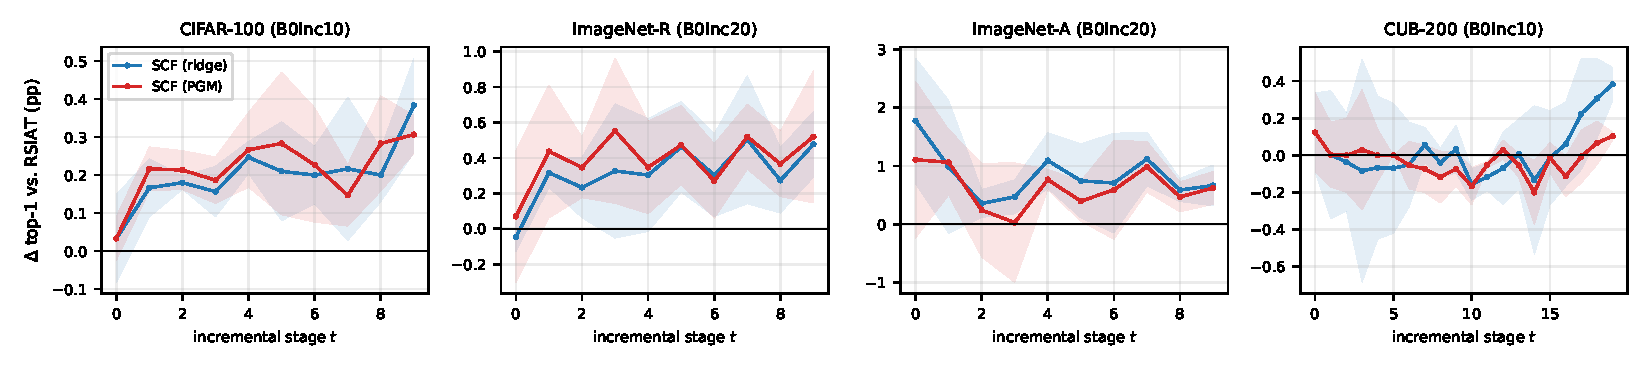
\includegraphics[width=\linewidth]{figures/delta_per_stage.pdf}
\caption{Top-1 difference to RSIAT at each stage, mean over runs. Solid:
fusion. Dotted: the generative score alone. Dashed: PGM with oracle states,
recomputed from old images (not exemplar-free). Every stand-alone generative
head falls further behind as tasks accumulate, and so does the oracle,
whereas both fusions stay above RSIAT.}
\label{fig:stage}
\end{figure}

\subsection{Analysis}
\label{sec:analysis}

\begin{table}[t]
\centering
\caption{Stand-alone heads: AIA difference to RSIAT over all 11 runs, and
paired contrasts with 95\% CI.}
\label{tab:heads}
\setlength{\tabcolsep}{5pt}
\begin{tabular}{lrr}
\toprule
Head (no fusion) & ImageNet-R & ImageNet-A \\
\midrule
Ridge on statistics, Eq.~\eqref{eq:ridge} & $-1.47$ & $-0.99$ \\
PGM, states from stale means & $-1.45$ & $-1.11$ \\
PGM, states from SSCA means, Eq.~\eqref{eq:state} & $-1.34$ & $-0.95$ \\
PGM, hierarchical & $-0.73$ & $-0.95$ \\
PGM, oracle states (control) & $-1.26$ & $-0.67$ \\
\midrule
\multicolumn{3}{l}{Paired contrasts (all runs, $n=11$)}\\
\quad SSCA means $-$ stale means & \multicolumn{2}{r}{$+0.13$ [0.08, 0.18]} \\
\quad hierarchical $-$ flat & \multicolumn{2}{r}{$+0.33$ [0.02, 0.64]} \\
\quad oracle $-$ stored states (final accuracy) & \multicolumn{2}{r}{$+0.64$ [0.48, 0.80]} \\
\bottomrule
\end{tabular}
\end{table}

\paragraph{Generative heads lose alone but help in fusion.}
Every stand-alone generative head is worse than RSIAT (Table~\ref{tab:heads}),
and the deficit grows with the number of tasks (Figure~\ref{fig:stage}). In
the base task, without drift, the PGM matches the linear head on
ImageNet-R ($-0.31$, $[-0.77,+0.15]$) and is ahead on ImageNet-A ($+1.6$).
These base-task figures come from a preliminary round with the same
networks, in which class states were built from per-sample features.
In that round, the two heads also made different errors. In the final stage
on ImageNet-R they disagree on $14\%$ of the test images:
\begin{itemize}
  \item the linear head is right on $5.8\%$ of the images,
  \item the PGM on $3.2\%$,
  \item neither on $5.4\%$.
\end{itemize}
The uncalibrated fusion corrected $0.7\%$ of the images and broke $0.4\%$.
Almost all of the corrections are cross-task errors of the linear head,
which is exactly the error type identified in Section~\ref{sec:gap}.

\paragraph{The calibration matters.}
Before calibration, the fusion summed the CA log-softmax and the PGM
log-probabilities with equal weight. It followed the linear head on $87\%$
of the disagreements and gained only $+0.25$ (ImageNet-R) and $+0.44$
(ImageNet-A). The reason is that the Born probabilities are much flatter
than a softmax with scale 50. The label-free scale $\kappa$ fixes this.
Across sources, the best weights are $0.25$--$1$, and all sources then give
$+0.45$ to $+0.62$ on held-out runs.

\paragraph{Better statistics are not the lever.}
\begin{itemize}
  \item States built from SSCA-updated means beat states from the means at
    learning time, but only by $+0.13$.
  \item Oracle states lift task~0 by $2.8$--$6.5$ points in every run, yet
    improve final accuracy by only $+0.64$, below the pre-registered
    threshold of $+1$.
  \item The oracle head itself still falls behind RSIAT as tasks accumulate
    (Figure~\ref{fig:stage}).
\end{itemize}
This agrees with Section~\ref{sec:gap}: improving drift compensation or
transporting the statistics would help little.

\paragraph{Exploratory: three sources.}
Fusing the linear head with both the ridge and the hierarchical PGM scores,
with weights chosen on the tuning group, gives $+0.71$
($[0.44, 0.97]$) on the held-out runs: $+0.40$ on ImageNet-R and $+0.90$ on
ImageNet-A. This combination was not pre-registered.
